\section{Results}
All results come from one full run over the \CountSketches{} sketches and \CountCommands{} commands (\ApiCalls{} cached model calls). Both systems use the same model, test cases and measurement code. Table~\ref{tab:headline} summarises every metric; the subsections discuss them. Differences on this test set are single-run, and several are small enough (a few commands out of 80) that we describe them as parity rather than wins.

\begin{table}[t]
\centering
\scriptsize
\caption{Headline results on the same 40 sketches and 80 commands (proposed vs.\ one-call baseline)}
\label{tab:headline}
\setlength{\tabcolsep}{3pt}
\begin{adjustbox}{max width=\columnwidth}
\begin{tabular}{lrrl}
\toprule
\textbf{Metric} & \textbf{Proposed} & \textbf{Baseline} & \textbf{Unit} \\
\midrule
Component detection F1 (analysis vs.\ baseline DOM) & 53.1 & 25.6 & \% \\
Component detection F1 (both on rendered DOM) & 42.9 & 25.6 & \% \\
Whisper word error rate & 4.0 & -- & \% \\
Voice command accuracy (from Whisper) & 91.2 & -- & \% \\
Visual similarity: layout IoU $\times$100 & 39.9 & 28.3 & IoU$\times$100 \\
Visual similarity: edge SSIM $\times$100 & 52.2 & 50.9 & SSIM$\times$100 \\
Functional correctness & 94.8 & 86.2 & \% \\
Requirement satisfaction & 87.5 & 86.0 & \% \\
Refinement success rate & 95.0 & 90.0 & \% \\
Preservation of unaffected components & 99.8 & 98.2 & \% \\
Validation pass rate before repair & 100.0 & -- & \% \\
Validation pass rate after repair & 100.0 & -- & \% \\
Injected faults detected & 96.8 & -- & \% \\
Injected faults repaired & 73.5 & -- & \% \\
Generation time, mean (s) & 15.5 & 24.0 & s \\
Modification time, mean (s) & 2.1 & 15.4 & s \\
Generated code parses & 100.0 & 100.0 & \% \\
ESLint messages per UI & 0.05 & 0.03 & count/UI \\
Component reuse ratio & 1.9 & 1.0 & usages/definition \\
Longest function (lines) & 105.6 & 206.1 & lines \\
\bottomrule
\end{tabular}
\end{adjustbox}
\end{table}


\subsection{Component Detection}
Table~\ref{tab:detection} separates the sketch-analysis stage from what is actually rendered. At the analysis stage, the hybrid detector reaches F1 \ComponentDetectionFOPipeline{}\% against \textbf{42.9\%} for OpenCV alone and \textbf{33.5\%} for the vision model alone, so neither component is sufficient. OpenCV localises well (mean IoU of matched boxes 0.72) but cannot read text or reliably tell types apart (type accuracy 52.9\%); the vision model labels well (87.7\% label accuracy) but localises loosely (mean IoU 0.52). Hybrid keeps OpenCV's boxes and the vision model's labels (95.3\% label accuracy).

The like-for-like comparison with the baseline is on the rendered DOM, because that is the only place the baseline's components exist. There the proposed pipeline scores F1 \ComponentDetectionFODomPipeline{}\% against \ComponentDetectionFODomBaseline{}\% for the baseline. A ground-truth oracle IR compiled by the same compiler scores 77.5\%, which bounds what the compiler achieves with perfect input and suggests that most of the remaining gap comes from upstream detection errors rather than code generation.

\begin{table*}[t]
\centering
\scriptsize
\caption{Component detection (micro-averaged; Hungarian matching, IoU $\geq$ 0.3, correct type)}
\label{tab:detection}
\setlength{\tabcolsep}{3.5pt}
\begin{adjustbox}{max width=\textwidth}
\begin{tabular}{lrrrrr}
\toprule
\textbf{Detector / output} & \textbf{Precision \%} & \textbf{Recall \%} & \textbf{F1 \%} & \textbf{Type acc. of matched \%} & \textbf{Mean IoU of matched} \\
\midrule
analysis: OpenCV only & 40.7 & 45.3 & 42.9 & 52.9 & 0.724 \\
analysis: Vision LLM only & 32.3 & 34.9 & 33.5 & 69.0 & 0.521 \\
analysis: Hybrid (CV + vision) & 48.9 & 58.2 & 53.1 & 68.1 & 0.717 \\
rendered DOM: Proposed (NeuroGenUI) & 40.6 & 45.5 & 42.9 & 82.3 & 0.580 \\
rendered DOM: Baseline (sketch$\rightarrow$AI$\rightarrow$UI) & 25.9 & 25.3 & 25.6 & 74.1 & 0.580 \\
rendered DOM: Oracle (GT IR) & 79.0 & 76.1 & 77.5 & 95.5 & 0.692 \\
\bottomrule
\end{tabular}
\end{adjustbox}
\end{table*}


\begin{figure}[t]
\centering
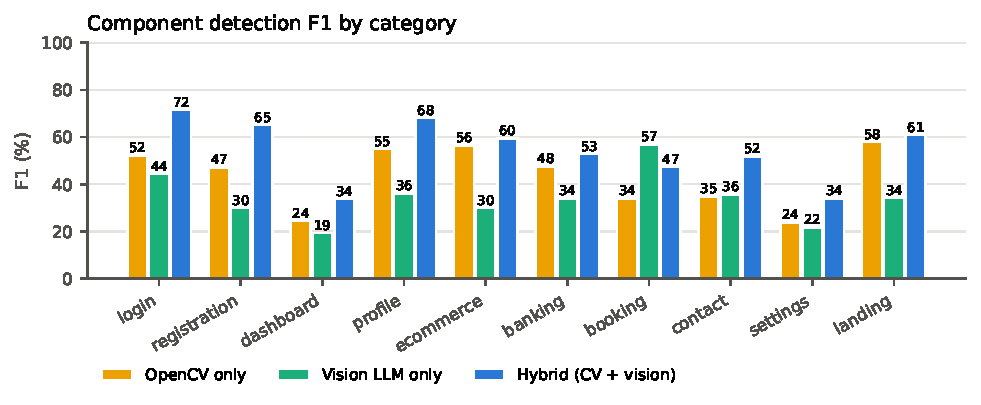
\includegraphics[width=\columnwidth]{figures/eval/detection_f1_by_category.pdf}
\caption{Detection F1 per screen category for each analysis mode and for the rendered DOM of both systems.}
\label{fig:detcat}
\end{figure}

\subsection{Voice Command Accuracy}
Whisper transcribes the synthesised commands with a corpus word error rate of \WhisperWerPipeline{}\%. From the Whisper transcript, \VoiceCommandAccuracyPipeline{}\% of commands are interpreted fully correctly (operation, target and parameters); from the reference text the figure is 93.8\% (Table~\ref{tab:voice}). Per category, add, remove, style, interaction and navigation are interpreted almost perfectly; resize is the weakest (60\% from the transcript) because quantities such as ``a bit bigger'' are ambiguous. Speech recognition errors cost about 2.6 percentage points relative to clean text (91.2\% vs.\ 93.8\%); we did not analyse which tokens were misrecognised.

\begin{table}[t]
\centering
\scriptsize
\caption{Voice command interpretation accuracy (\%)}
\label{tab:voice}
\setlength{\tabcolsep}{3.5pt}
\begin{adjustbox}{max width=\columnwidth}
\begin{tabular}{lrrrrr}
\toprule
\textbf{Input} & \textbf{Commands} & \textbf{Op type} & \textbf{Target} & \textbf{Parameters} & \textbf{All correct} \\
\midrule
Ground-truth text & 80 & 97.5 & 97.5 & 98.6 & 93.8 \\
Whisper transcript & 80 & 96.2 & 97.5 & 95.7 & 91.2 \\
\bottomrule
\end{tabular}
\end{adjustbox}
\end{table}


\subsection{Generated UI Quality}
Table~\ref{tab:quality} reports visual and functional quality. The generated UI renders in 100\% of cases for both systems. Layout IoU against the sketch is 0.399 for the proposed pipeline and 0.283 for the baseline; the compiler's oracle ceiling is 0.593. Edge SSIM is nearly identical (0.52 vs.\ 0.51), so the two systems look equally similar to the sketch at the pixel-structure level; the gain is in component placement. Functional correctness is \FunctionalCorrectnessPipeline{}\% vs.\ \FunctionalCorrectnessBaseline{}\%, and the difference is almost entirely in navigation (92\% vs.\ 72\% of 25 specified interactions). Validation and message behaviours are equal. Requirement satisfaction is at parity (\RequirementSatisfactionPipeline{}\% vs.\ \RequirementSatisfactionBaseline{}\%); the baseline is better at honouring specific input types (97.1\% vs.\ 91.2\%).

\begin{table*}[t]
\centering
\scriptsize
\caption{Generated UI quality: visual similarity, functional correctness, requirement satisfaction}
\label{tab:quality}
\setlength{\tabcolsep}{3.5pt}
\begin{adjustbox}{max width=\textwidth}
\begin{tabular}{lrrrrrr}
\toprule
\textbf{System} & \textbf{Sketches} & \textbf{Renders \%} & \textbf{Layout IoU} & \textbf{Edge SSIM} & \textbf{Functional \% (n)} & \textbf{Requirements \% (n)} \\
\midrule
Proposed (NeuroGenUI) & 40 & 100.0 & 0.399 & 0.522 & 94.8 (58) & 87.5 (407) \\
Proposed, before repair & 40 & 100.0 & 0.399 & 0.522 & 94.8 (58) & 87.5 (407) \\
Baseline (sketch$\rightarrow$AI$\rightarrow$UI) & 40 & 100.0 & 0.283 & 0.509 & 86.2 (58) & 86.0 (407) \\
Oracle (GT IR) & 40 & 100.0 & 0.593 & 0.551 & 6.9 (58) & 85.3 (407) \\
\bottomrule
\end{tabular}
\end{adjustbox}
\end{table*}


\begin{figure}[t]
\centering
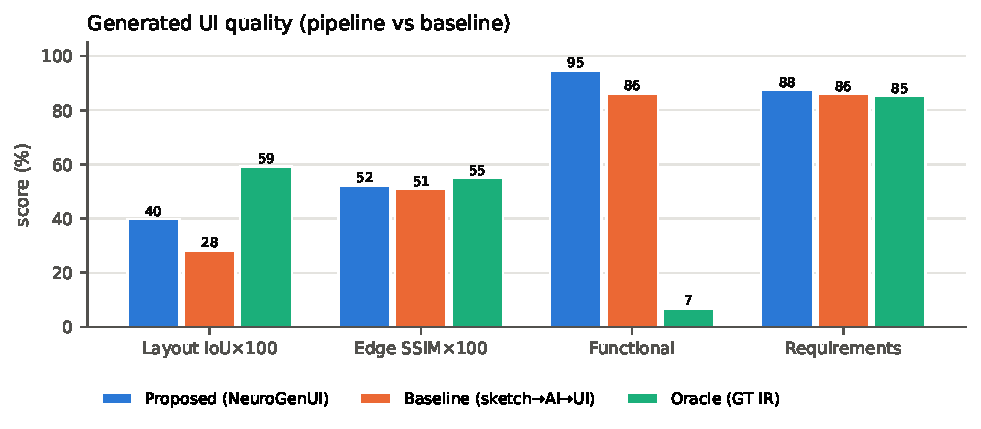
\includegraphics[width=\columnwidth]{figures/eval/generation_quality.pdf}
\caption{Generated UI quality: pipeline, baseline and the ground-truth oracle.}
\label{fig:quality}
\end{figure}

\subsection{Voice-Guided Refinement}
Table~\ref{tab:refine} shows refinement success and preservation per command category. The proposed pipeline applies \RefinementSuccessRatePipeline{}\% of commands successfully against \RefinementSuccessRateBaseline{}\% for the baseline (93.8\% when the command goes through Whisper), a difference of four commands out of 80 that we do not claim as significant. The categories differ: the pipeline is better on add, style, navigation and resize; the baseline is better on modify and move (100\% on both). The clearer difference is preservation. Because refinements are operations on the existing IR, \PreservationRatePipeline{}\% of unaffected components are unchanged in type, text, colour, size and font, against \PreservationRateBaseline{}\% when the baseline regenerates the program. Latency differs by an order of magnitude: \ModificationTimeMsPipeline{}\,s on average for the pipeline (one short interpretation call plus deterministic edit and compile) against \ModificationTimeMsBaseline{}\,s for a full regeneration.

\begin{table*}[t]
\centering
\scriptsize
\caption{Refinement success and preservation (\%) per command category}
\label{tab:refine}
\setlength{\tabcolsep}{3.5pt}
\begin{adjustbox}{max width=\textwidth}
\begin{tabular}{lrrrrrr}
\toprule
\textbf{Category} & \textbf{Success: Proposed (NeuroGenUI)} & \textbf{Success: Proposed, Whisper transcript} & \textbf{Success: Baseline (sketch$\rightarrow$AI$\rightarrow$UI)} & \textbf{Preserved: Proposed (NeuroGenUI)} & \textbf{Preserved: Proposed, Whisper transcript} & \textbf{Preserved: Baseline (sketch$\rightarrow$AI$\rightarrow$UI)} \\
\midrule
add & 100.0 & 100.0 & 80.0 & 100.0 & 100.0 & 96.3 \\
remove & 100.0 & 100.0 & 100.0 & 99.4 & 99.4 & 98.9 \\
modify & 90.0 & 90.0 & 100.0 & 100.0 & 100.0 & 100.0 \\
move & 80.0 & 80.0 & 100.0 & 100.0 & 100.0 & 94.1 \\
resize & 90.0 & 80.0 & 70.0 & 99.1 & 98.2 & 99.2 \\
style & 100.0 & 100.0 & 90.0 & 100.0 & 100.0 & 97.1 \\
interaction & 100.0 & 100.0 & 100.0 & 100.0 & 100.0 & 100.0 \\
navigation & 100.0 & 100.0 & 80.0 & 100.0 & 100.0 & 100.0 \\
all & 95.0 & 93.8 & 90.0 & 99.8 & 99.7 & 98.2 \\
\bottomrule
\end{tabular}
\end{adjustbox}
\end{table*}


\subsection{Validation and Repair}
After the development fixes described in Section~\ref{sec:dev}, \ValidationPassRateBeforeRepairPipeline{}\% of generated UIs pass validation before repair, so on this test set the repair loop is not triggered during normal generation and we cannot measure a pass-rate improvement. We therefore evaluate validation and repair directly by \emph{fault injection} (Table~\ref{tab:faults}): across 438 injected faults on pipeline and oracle UIs, the validator detects \FaultDetectionRatePipeline{}\% and the repair loop restores \FaultRepairRatePipeline{}\%. Detection is strong for hidden, zero-size, reordered and broken-event faults. Repair is reliable for broken event handlers (100\%) and reordering (97.5\%) but weak for hidden nodes (42.5\% on pipeline UIs) and deleted nodes (55\%), so the loop is not a general recovery mechanism. Deleting a node is also the fault the validator detects least often on pipeline UIs (75\%); we did not investigate why.

\begin{table}[t]
\centering
\scriptsize
\caption{Fault injection: validator detection and repair recovery (\%)}
\label{tab:faults}
\setlength{\tabcolsep}{3.5pt}
\begin{adjustbox}{max width=\columnwidth}
\begin{tabular}{lrrrrr}
\toprule
\textbf{IR source} & \textbf{Fault} & \textbf{Cases} & \textbf{Detected \%} & \textbf{Localised \%} & \textbf{Repaired \%} \\
\midrule
oracle & delete\_node & 40 & 95.0 & 95.0 & 77.5 \\
oracle & hide\_node & 40 & 100.0 & 100.0 & 52.5 \\
oracle & zero\_size & 40 & 100.0 & 100.0 & 65.0 \\
oracle & swap\_order & 40 & 100.0 & 62.5 & 97.5 \\
oracle & code\_error & 40 & 100.0 & 100.0 & None \\
oracle & all & 200 & 99.0 & 91.5 & 73.1 \\
pipeline & delete\_node & 40 & 75.0 & 60.0 & 55.0 \\
pipeline & hide\_node & 40 & 100.0 & 100.0 & 42.5 \\
pipeline & zero\_size & 40 & 95.0 & 95.0 & 75.0 \\
pipeline & swap\_order & 40 & 100.0 & 50.0 & 97.5 \\
pipeline & break\_event & 38 & 100.0 & 100.0 & 100.0 \\
pipeline & code\_error & 40 & 100.0 & 100.0 & None \\
pipeline & all & 238 & 95.0 & 84.0 & 73.7 \\
\bottomrule
\end{tabular}
\end{adjustbox}
\end{table}


\begin{figure}[t]
\centering
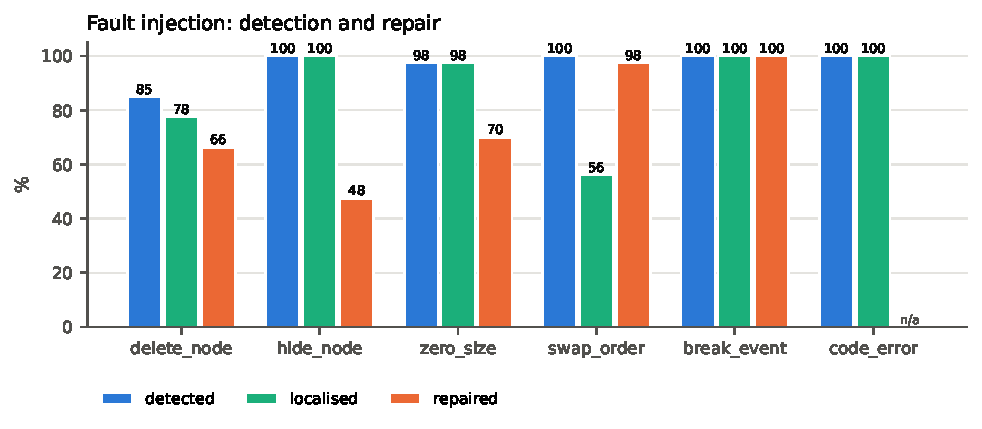
\includegraphics[width=\columnwidth]{figures/eval/fault_injection.pdf}
\caption{Fault injection: share of injected faults detected, localised and repaired, by fault type.}
\label{fig:faults}
\end{figure}

\subsection{Generation Time}
The proposed pipeline produces a usable UI in \GenerationTimeMsPipeline{}\,s on average (median 10.7\,s) against \GenerationTimeMsBaseline{}\,s for the baseline, including validation and repair (16.4\,s). Table~\ref{tab:latency} breaks this down: sketch analysis (10.4\,s mean, dominated by the vision call) and interpretation (5.1\,s) account for almost all of it, while fusion, code generation and validation together take about 0.5\,s. Latencies include network time to the model API and vary with load.

\begin{table}[t]
\centering
\scriptsize
\caption{Latency per stage (ms)}
\label{tab:latency}
\setlength{\tabcolsep}{3.5pt}
\begin{adjustbox}{max width=\columnwidth}
\begin{tabular}{lrrrrr}
\toprule
\textbf{System} & \textbf{Stage} & \textbf{n} & \textbf{Mean} & \textbf{Median} & \textbf{p95} \\
\midrule
pipeline & analyze\_sketch & 40 & 10350 & 5890 & 10705 \\
pipeline & interpret & 40 & 5114 & 4987 & 7215 \\
pipeline & fuse & 40 & 3 & 3 & 6 \\
pipeline & codegen & 40 & 1 & 1 & 2 \\
pipeline & total\_generate & 40 & 15469 & 10654 & 18343 \\
pipeline & validate & 40 & 517 & 443 & 703 \\
pipeline & repair & 40 & 460 & 442 & 667 \\
pipeline & total\_with\_validation & 40 & 16446 & 11563 & 19432 \\
baseline & total\_generate & 40 & 23968 & 16976 & 65240 \\
analyze\_cv & analyze\_cv & 40 & 66 & 55 & 103 \\
analyze\_vision & analyze\_vision & 40 & 6445 & 6237 & 8711 \\
analyze\_hybrid & analyze\_hybrid & 40 & 10350 & 5890 & 10705 \\
pipeline & modify\_total & 80 & 2103 & 2063 & 2708 \\
pipeline\_voice & modify\_total & 80 & 2104 & 2106 & 2676 \\
baseline & modify\_total & 80 & 15360 & 13883 & 23314 \\
\bottomrule
\end{tabular}
\end{adjustbox}
\end{table}


\subsection{Code Quality}
Both systems produce code that parses in all cases (Table~\ref{tab:code}). Generated code from the proposed compiler is organised in reusable components: each definition is used 1.85 times on average against 1.01 for the baseline, which inlines most elements. The baseline's longest function averages 206 lines against 106 for the proposed code, and the exported project is split into multiple files. ESLint reports almost no messages for either system (0.05 vs.\ 0.03 per UI). The compiler's longest function grew from 57 to 106 lines between the development run and the final run, after geometry-aware layout was added.

\begin{table*}[t]
\centering
\scriptsize
\caption{Static code quality of the generated React (mean per UI)}
\label{tab:code}
\setlength{\tabcolsep}{3.5pt}
\begin{adjustbox}{max width=\textwidth}
\begin{tabular}{lrrrrrrrr}
\toprule
\textbf{Code} & \textbf{UIs} & \textbf{Parses \%} & \textbf{LOC} & \textbf{Components} & \textbf{Reuse ratio} & \textbf{Max function lines} & \textbf{ESLint msgs} & \textbf{Files} \\
\midrule
Proposed (NeuroGenUI) [project] & 40 & 100.0 & 410.8 & 13.9 & 1.85 & 105.6 & 0.0 & 17.9 \\
Proposed (NeuroGenUI) [preview] & 40 & 100.0 & 379.0 & 13.9 & 1.85 & 105.6 & 0.1 & 1.0 \\
Baseline (sketch$\rightarrow$AI$\rightarrow$UI) [preview] & 40 & 100.0 & 246.3 & 1.4 & 1.01 & 206.1 & 0.0 & 1.0 \\
Oracle (GT IR) [preview] & 40 & 100.0 & 307.6 & 11.6 & 1.60 & 76.1 & 1.0 & 1.0 \\
\bottomrule
\end{tabular}
\end{adjustbox}
\end{table*}

